 \documentclass{standalone}
 \usepackage{tikz}
\usepackage{tkz-graph}
 \begin{document}
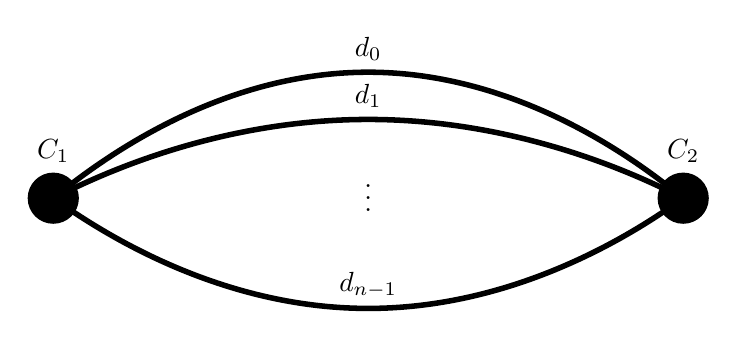
\begin{tikzpicture}
    \SetGraphUnit{5}
      \node[black] at (8,5.9) {$d_0$};
       \node[black] at (4,4.6) {$C_1$};
        \node[black] at (12,4.6) {$C_2$};
         \node[black] at (8,5.3) {$d_1$};
            \node[black] at (8,2.9) {$d_{n-1}$};
            \node[black] at (8,4.15) {.};
            \node[black] at (8,4.0) {.};
            \node[black] at (8,3.85) {.};
  \tikzstyle{VertexStyle}=[shape = circle, draw, minimum size = 10pt]
  \SetUpVertex[FillColor=black]  
  \Vertex[x=4,y=4]{1}
  \Vertex[x=12,y=4]{2}  
 \draw[->,line width=2pt,black] (4,4) parabola bend (8,5.6) (12,4);
  \draw[->,line width=2pt,black] (4,4) parabola bend (8,5) (12,4);
      \draw[->,line width=2pt,black] (4,4) parabola bend (8,2.6) (12,4);
\end{tikzpicture}
 \end{document}